%% SECTION 4.3 %%
\section{Shattering}
\label{sec: shattering}

The sets of vectors that interest us in the definition of Rademacher complexity of
$\mathcal{A}$ are sets of the form
\begin{equation}
\label{eq: T(z)}
    \highlightMath{
        T(z) = \{(\indSet{z_1 \in A}, \dots, \indSet{z_n \in A})^{\top} \with A \in \mathcal{A}\},
    }
\end{equation}
for $z = (z_1, \dots, z_n) \in \mathcal{Z}^n$, where\footnote{Again, this definition makes sense for arbitrary spaces $\mathcal{Z}$, i.e., we can take a family of sets $\mathcal{A}$ and $z = (z_1, \dots, z_n) \in \mathcal{Z}^n$ and then define $T(z)$ as above.} $z_i \in \mathcal{X} \times \set{0, 1}$. Particularly, the cardinality of $T(z)$, i.e., the number of binary patterns a tuple of points $(z_1, \dots, z_n)$ can replicate as $A$ ranges over the family of sets $\mathcal{A}$, will be extremely important, as it will arise when trying to control the Rademacher complexity of $\mathcal{A}$. A first hint at this is the following result, which allows us to link the Rademacher complexity of $\mathcal{A}$ to the Rademacher complexity of the sets $T(z)$:

\begin{lemma}
\label{lem: rademacher complexity of family of sets}
The Rademacher complexity of a family of sets $\mathcal{A}$ in a space $\mathcal{Z}$ satisfies
\[
    \mathfrak{R}_n(\mathcal{A}) = \sup_{z \in \mathcal{Z}^n} \mathfrak{R}_n(T(z)).
\]
\end{lemma}

\begin{proof}
This is straightforward: by the definition of the set $T(z)$ in \eqref{eq: T(z)}, we have
\[
    \sup_{z \in \mathcal{Z}^n} \mathfrak{R}_n(T(z)) = \sup_{z \in \mathcal{Z}^n} \Exp\left[\sup_{b \in T(z)} \abs{\frac{1}{n} \sum_{i=1}^n \sigma_i b_i}\right] = \sup_{z \in \mathcal{Z}^n} \Exp\left[\sup_{A \in \mathcal{A}} \abs{\frac{1}{n} \sum_{i=1}^n \sigma_i \indSet{z_i \in A}}\right] = \mathfrak{R}_n(\mathcal{A}). \qedhere
\]
\end{proof}

Let us briefly investigate the set $T(z)$ and its cardinality to get a better understanding. First, even though the cardinality of $\mathcal{A}$ can be infinite, the cardinality of $T(z)$ is at most $2^n$. To further illustrate the concept, let us look at an example: for the set $z = \set{z_1, z_2, z_3, z_4}$, the binary pattern $(1, 1, 0, 1)$ is contained in $T(z)$ if and only if there exists some set $A \in \mathcal{A}$ such that $z \cap A = \set{z_1, z_2, z_4}$, i.e., the set of points $\set {z_1, z_2, z_4}$ can be separated from the remaining points in $z$ by a set $A$ in $\mathcal{A}$. In this case, the set of points $\set{z_1, z_2, z_4}$ is said to be \emph{picked up} by $\mathcal{A}$. Hence, the cardinality of $T(z)$ equals the number of elements of the power set $\power(z)$ that can be picked up by $\mathcal{A}$, i.e.,
\[
    \highlightMath{
        \abs{T(z)} = \abs{z \cap \mathcal{A}},
    }
\]
where
\[
    z \cap \mathcal{A} = \set{z \cap A \with A \in \mathcal{A}}.
\]
This leads to the following definition:

\begin{definition}
A family of sets $\mathcal{A}$ \emph{shatters} the set of points $z = \set{z_1, \dots, z_n}$, if
\[
    \abs{T(z)} = \abs{z \cap \mathcal{A}} = 2^n.
\]
\end{definition}

Clearly, a family of sets $\mathcal{A}$ shatters the set of points $\set{z_1, \dots, z_n}$ if and only if \emph{every} subset of $z$ can be picked up by $\mathcal{A}$. Recall that the set of points we are interested in are i.i.d.\ realizations $Z_1, \dots, Z_n$ of $Z = (X, Y)$. As the distribution of $Z$ is unknown, these realizations may theoretically take on any value over the sample space $\mathcal{Z} = \mathcal{X} \times \set{0, 1}$. Hence, we define the \emph{shatter coefficients} of a family of sets $\mathcal{A}$ as follows:

\begin{definition}
The \emph{$n$-th shatter coefficient} $\mathcal{S}_{\mathcal{A}}(n)$ of a family of sets $\mathcal{A}$ is given by
\[
    \mathcal{S}_{\mathcal{A}}(n) = \sup_{z \in \mathcal{Z}^n} \abs{T(z)} = \sup_{z \in \mathcal{Z}^n} \abs{z \cap \mathcal{A}}.
\]
\end{definition}

By definition, $\mathcal{S}_{\mathcal{A}}(n) = 2^n$ if $\mathcal{A}$ shatters a set $\set{z_1, \dots, z_n} \subset \mathcal{Z}$, i.e., if there exists a set $z = \set{z_1, \dots, z_n}$ such that every subset of $z$ can be picked up by $\mathcal{A}$. Analogously, we have $\mathcal{S}_{\mathcal{A}}(n) < 2^n$ if \emph{no} set of points $\set{z_1, \dots, z_n}$ can be shattered by $\mathcal{A}$. The largest integer $k$ for which there still exists a set that can be shattered by $\mathcal{A}$ is precisely the \emph{Vapnik-Chervonenkis dimension} of $\mathcal{A}$:

\begin{definition}
The \emph{Vapnik-Chervonenkis dimension} $\VC(\mathcal{A})$ of a family of sets $\mathcal{A}$ is the largest integer $k$ such that $\mathcal{S}_{\mathcal{A}}(k) = 2^k$. If $\mathcal{S}_{\mathcal{A}}(n) = 2^n$ holds for all $n$, we set $\VC(\mathcal{A}) = \infty$.
\end{definition}

Note that this definition only makes sense if $\mathcal{S}_{\mathcal{A}}(n) < 2^n$ implies $\mathcal{S}_{\mathcal{A}}(m) < 2^m$ for all $m > n$, which indeed is true. Hence, $\VC(\mathcal{A}) = d$ implies that for every integer $n = 1, \dots, d$, there exists \emph{at least one} set $\set{z_1, \dots, z_n}$ that $\mathcal{A}$ shatters, but there exist \emph{no} sets of cardinality $m > d$ that $\mathcal{A}$ shatters. We will see that the VC dimension will play a role similar to the cardinality of sets, but on an exponential scale.

\begin{figure}
    \centering
    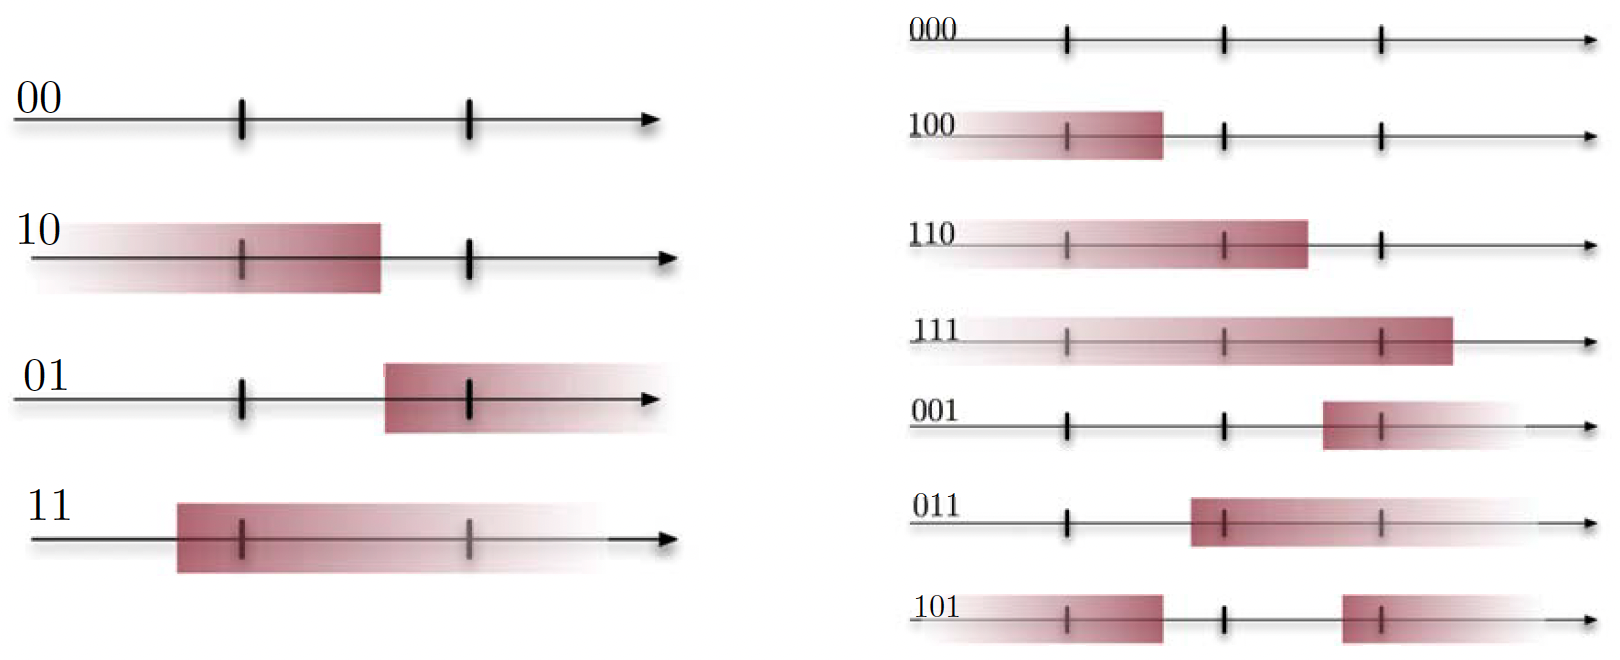
\includegraphics[width=0.8\textwidth]{mit-ocw/half-lines}
    \caption{%
        The family $\mathcal{A} = \set{(-\infty, a] \with a \in \R} \cup \set{[a, \infty) \with a \in \R}$ of half-lines shatters every set of cardinality $2$, but \emph{no} set of three points. In particular, $\VC(\mathcal{A}) = 2$. Note that the binary pattern $101$ (bottom right) can only be created if one extends the family $\mathcal{A}$ to also include unions of half-lines. \\
        \indent\emph{Note}. From \say{Mathematics of Machine Learning (18.657),} by P.~Rigollet, Fall 2015, \emph{Massachusetts Institute of Technology: MIT OpenCouseWare}, p.~29 (\url{https://ocw.mit.edu/}). \href{https://creativecommons.org/licenses/by-nc-sa/4.0/}{CC BY-NC-SA 4.0}.
    }
    \label{fig: VC dimension of half-lines}
\end{figure}

Let us consider an example to get a better understanding of all of the terms introduced in this section. Take, for example, $\mathcal{A} = \set{(-\infty, a] \with a \in \R} \cup \set{[a, \infty) \with a \in \R}$ to be the set of half-lines, and let our sample space be the real line $\R$. Clearly, $\abs{\mathcal{A}} = \infty$. As it turns out, we can shatter every set of two points $\set{z_1, z_2}$: WLOG, assume $z_1 < z_2$ and let $\varepsilon = (z_2 - z_1)/2 > 0$. Then,
\begin{itemize}
    \item $A = (-\infty, z_1 - 1]$ picks up the empty set,

    \item $A = (-\infty, z_1 + \varepsilon]$ picks up the set $\set{z_1}$,

    \item $A = [z_1 + \varepsilon, \infty)$ picks up the set $\set{z_2}$,

    \item $A = [z_1 - 1, \infty)$ picks up the set $\set{z_1, z_2}$.
\end{itemize}
In particular, $\mathcal{A}$ shatters the set $\set{z_1, z_2}$, and we can conclude that\footnote{Note that, by definition, $\mathcal{A}$ need only shatter a single set of two points for the identity $\mathcal{S}_{\mathcal{A}}(2) = 2^2$ to hold!} $\mathcal{S}_{\mathcal{A}}(2) = 2^2$, and hence $\VC(\mathcal{A}) \geq 2$. However, $\mathcal{A}$ shatters \emph{no} set of three points $\set{z_1, z_2, z_3}$: WLOG, we can assume $z_1 < z_2 < z_3$. In this case, the set $\set{z_2}$ cannot be picked up by $\mathcal{A}$! This is easy to see: let $A \in \mathcal{A}$ be a set such that $z_2 \in A$. This implies that $A = (-\infty, z_2 + \delta]$ or $A = [z_2 - \delta, \infty)$ with $\delta \geq 0$. However, we have $z_1 \in (-\infty, z_2 + \delta]$ and $z_3 \in [z_2 - \delta, \infty)$, i.e., it is impossible to pick up the singleton $\set{z_2}$ with half-lines! More generally, one can show that half-lines can only generate binary patterns with ones followed by zeros or zeros followed by ones but they cannot generate alternating patterns like 010 or 101. In particular, $\mathcal{S}_{\mathcal{A}}(n) = 2n < n^2$ for $n > 2$.

Let us discuss another example. Let $\mathcal{A}$ be the set of hyperrectangles in $\R^d$, i.e., $\mathcal{A} = \set{[\mathbf{a}, \mathbf{b}] \with \mathbf{a}, \mathbf{b} \in \R^d}$, where
\[
    [\mathbf{a}, \mathbf{b}] = \prod_{i=1}^d [a^{(i)}, b^{(i)}] = \{(x^{(1)}, \dots, x^{(d)}) \in \R^d \with x^{(i)} \in [a^{(i)}, b^{(i)}] \text{ for } i = 1, \dots, d\}
\]
with $\mathbf{a} = (a^{(1)}, \dots, a^{(d)})^{\top}$ and $\mathbf{b} = (b^{(1)}, \dots, b^{(d)})^{\top}$ such that $a^{(i)} \leq b^{(i)}$ for all $i = 1, \dots, d$. For $d=2$, the family $\mathcal{A}$ shatters the set $\{(1, 0)^{\top}, (0, 1)^{\top}, (-1, 0)^{\top}, (0, -1)^{\top}\}$ of four points in $\R^2$, and, more generally, one can show that $\mathcal{A}$ always shatters a set of $2d$ points for arbitrary dimensions $d$. This tells us that $\mathcal{S}_{\mathcal{A}}(2d) = 2^{2d}$ and $\VC(\mathcal{A}) \geq 2d$. However, the family $\mathcal{A}$ can never shatter a set of $2d + 1$ points. The argument is similar in spirit to the one made earlier for half-lines. Let $B = \set{x_1, \dots, x_{2d+1}}$ be a set of $2d + 1$ points and define points $y_1, \dots, y_d$ and $z_1, \dots, z_d$ as follows:
\[
    y_i = \argmin_{x_j \in B} x_j^{(i)}, \qquad z_i = \argmax_{x_j \in B} x_j^{(i)}, \qquad i = 1, \dots, d.
\]
With these definitions, any set that contains $\set{y_1, \dots, y_d, z_1, \dots, z_d}$, will inevitably contain the entire set $B$. Hence, it is impossible to pick up the set $\set{y_1, \dots, y_d, z_1, \dots, z_d}$ and $\mathcal{S}_{\mathcal{A}}(2d + 1) < 2^{2d + 1}$. Consequently, $\VC(\mathcal{A}) = 2d$.
